\documentclass{reportx}

\NewDocumentCommand\optmodule{sO{}mmm}{%
    \IfBooleanTF{#1}{%
        \begin{equation*}
            \ifthenelse{\equal{#2}{}}{}{(#2)\quad}
            \begin{aligned}
                \begin{cases}
                    #3 \quad & #4 \\
                    \mathrm{s.t.} \quad #5
                \end{cases}
            \end{aligned}
        \end{equation*}
    }{%
        \begin{equation}
            \ifthenelse{\equal{#2}{}}{}{(#2)\quad}
            \begin{aligned}
                \begin{cases}
                    #3 \quad & #4 \\
                    \mathrm{s.t.} \quad #5
                \end{cases}
            \end{aligned}
        \end{equation}
    }%
}

\begin{document}
    \section{实验内容}

本实验将进行如下工作:

第一, 介绍各种典型的优化方法.
将系统地梳理优化算法的基本分类与原理, 涵盖从无需梯度信息的无导数优化方法到依赖梯度信息的有导数优化方法.
在一阶优化器部分, 将重点讲解基于梯度信息的优化策略, 包括最基本的梯度下降法、适用于非光滑目标函数的次梯度下降法, 以及加速收敛的共轭方向法、共轭梯度法和采用迭代更新Hessian矩阵近似的变尺度法(如BFGS法).
二阶优化器则引入目标函数的Hessian矩阵以提升收敛速度, 典型方法包括Newton法与其改进形式阻尼Newton法, 后者通过调整Hessian矩阵提升算法稳定性.
此外, 还将介绍交替方向乘子法(ADMM)这种适用于分布式和约束优化问题的有效算法, 以及Krylov子空间方法等在高维大规模问题中应用广泛的迭代式优化策略.

第二, 实现上述优化方法.
利用Python编程语言实现所介绍的各类优化算法.
为了确保每种方法具有通用性和可扩展性, 将使用PyTorch框架对各种优化器进行实现, 继承Optimizer接口, 便于后续在不同类型的目标函数上进行测试和比较.

第三, 测试上述优化方法.
使用一个典型的测试函数对各优化器进行性能评估——Rosenbrock函数.
实验将对每种优化器在在相同初始点下的收敛过程进行可视化分析, 并对优化器性能进行比较.

    \section{优化方法介绍}

\subsection{随机搜索法}

随机搜索法(Random Search Method)是一种无导数优化方法,其基本思想是在定义域内随机生成若干点,并选择函数值最小的作为当前最优解。
设优化问题为
\begin{equation*}
    \min_{\bm{x}\in\mathbb{R}^n} ~ f(\bm{x}) \text{。}
\end{equation*}
在第$k$次迭代中,随机生成点$\bm{x}_k'\in U(\bm{x}_k)$,其中$U(\bm{x}_k)$为$\bm{x}_k$的某一邻域。

则有迭代公式
\begin{equation*}
    \bm{x}_{k+1}=\bm{x}_k'
    \begin{cases}
        \bm{x}_k'\text{,} &f(\bm{x}_k')<f(\bm{x}_k) \text{,} \\
        \bm{x}_k\text{,} &f(\bm{x}_k')\geq f(\bm{x}_k) \text{。}
    \end{cases}
\end{equation*}
该方法通过不断试探更新寻找函数值更小的位置,而无需任何梯度信息。

\subsection{梯度下降法}

梯度下降法(Gradient Descent Method)利用目标函数的梯度信息,以梯度的负方向作为下降方向,即
\begin{equation*}
    \bm{x}_{k+1}=\bm{x}_k-\alpha_k\nabla f(\bm{x}_k) \text{,}
\end{equation*}
其中$\alpha_k>0$为学习率,$\nabla f(\bm{x}_k)$为目标函数在点$\bm{x}_k$处的梯度。

\subsection{次梯度下降法}

次梯度下降法(Subgradient Descent Method)用于优化非光滑凸函数。
若$f$在点$\bm{x}_k$处不可导,但存在次梯度$\bm{g}_k\in\partial f(\bm{x}_k)$, 则有
\begin{equation*}
    \bm{x}_{k+1}=\bm{x}_k-\alpha_k\bm{g}_k \text{,}
\end{equation*}
其中$\alpha_k>0$为学习率,$\partial f(\bm{x}_k)$为目标函数在点$\bm{x}_k$处的次梯度集合。

\subsection{共轭方向法}

共轭方向法(Conjugate Direction Method)用于二次函数
\begin{equation*}
    f(\bm{x})=\frac{1}{2}\bm{x}^\mathrm{T}\bm{Ax}-\bm{b}^\mathrm{T}\bm{x} \text{,}
\end{equation*}
其中矩阵$\bm{A}$对称正定。

共轭方向法需要构造一组关于矩阵$\bm{A}$的共轭方向$\{\bm{d}_i\}_{i=1}^n$,使得
\begin{equation*}
    \bm{d}_i\bm{A}\bm{d}_j=0 \text{,} i\ne j \text{,}
\end{equation*}
沿着这些方向进行线性搜索,即
\begin{equation*}
    \bm{x}_{k+1}=\bm{x}_k-\alpha_k\bm{d}_k \text{,}
\end{equation*}
其中$\alpha_k>0$为学习率,可通过一维搜索得到。

\subsection{共轭梯度法}

共轭梯度法(Conjugate Gradient Method)是一种特殊的共轭方向法,使用当前梯度和上一次方向构造共轭方向,避免计算$\bm{A}$。
对于二次函数,其迭代格式为:
\begin{align*}
    &\bm{x}_{k+1}=\bm{x}_k-\alpha_k\bm{d}_k \text{,} \\
    &\alpha_k=\frac{\bm{r}_k^\mathrm{T}\bm{r}_k}{\bm{d}_k^\mathrm{T}\bm{Ad}_k} \text{,} \\
    &\bm{d}_k=\bm{r}_k+\beta_{k-1}\bm{d}_{k-1} \text{,} \beta_{k-1}=\frac{\bm{r}_k^\mathrm{T}\bm{r}_k}{\bm{r}_{k-1}^\mathrm{T}\bm{r}_{k-1}} \text{,} \\
    &\bm{r}_k=\bm{b}-\bm{Ax}_k \text{,} \bm{r}_0=-\nabla f(\bm{x}_0) \text{。}
\end{align*}

    \section{实验设置及结果}

为了使优化器的通用性和可扩展性,实验基于PyTorch的Optimizer类进行优化器实现,并分别实现了随机搜索优化器,梯度下降优化器,次梯度下降优化器,共轭方向优化器,共轭梯度优化器,变尺度法优化器(BFGS),随机梯度下降优化器,Newton优化器,阻尼Newton优化器,ADMM优化器和Krylov子空间优化器,并使用Rosenbrock Banana函数作为优化器测试函数,即
\begin{equation*}
    f(x_1, x_2)=(a-x_1)^2-b(x_2-x_1^2)^2 \text{,}
\end{equation*}
其中$a=1$,$b=-100$。
实验结果如\cref{table:result}所示,各优化器的最优值收敛曲线和最优点收敛路径如\cref{figure:random search}至\cref{figure:krylov}所示。

\begin{table}[ht]
    \centering
    \caption{实验结果}
    \label{table:result}
    \begin{tabular}{cccc}
        \toprule
        \textbf{优化器} & \textbf{最优点} & \textbf{最优值} & \textbf{迭代轮次} \\
        \midrule
        Random Search & $(1.00, 1.00)$ & 0.00 & 1326 \\
        Gradient Descent & $(0.99, 1.00)$ & 0.00 & 10808 \\
        Subgradient Descent & $(0.99, 1.00)$ & 0.00 & 10808 \\
        Conjugate Direction & $(1.00, 1.00)$ & 0.00 & 23366 \\
        Conjugate Gradient & $(1.00, 1.00)$ & 0.00 & 500 \\
        BFGS & $(1.00, 1.00)$ & 0.00 & 21983 \\
        SGD & $(1.00, 1.00)$ & 0.00 & 6350 \\
        Newton & $(1.00, 1.00)$ & 0.00 & 7 \\
        Damped Newton & $(1.00, 1.00)$ & 0.00 & 2970 \\
        ADMM & $(1.00, 1.00)$ & 0.00 & 22184 \\
        Krylov & $(1.00, 1.00)$ & 0.00 & 6385 \\
        \bottomrule
    \end{tabular}
\end{table}

\begin{figure}[!ht]
    \centering
    \begin{subfigure}{0.4\textwidth}
        \centering
        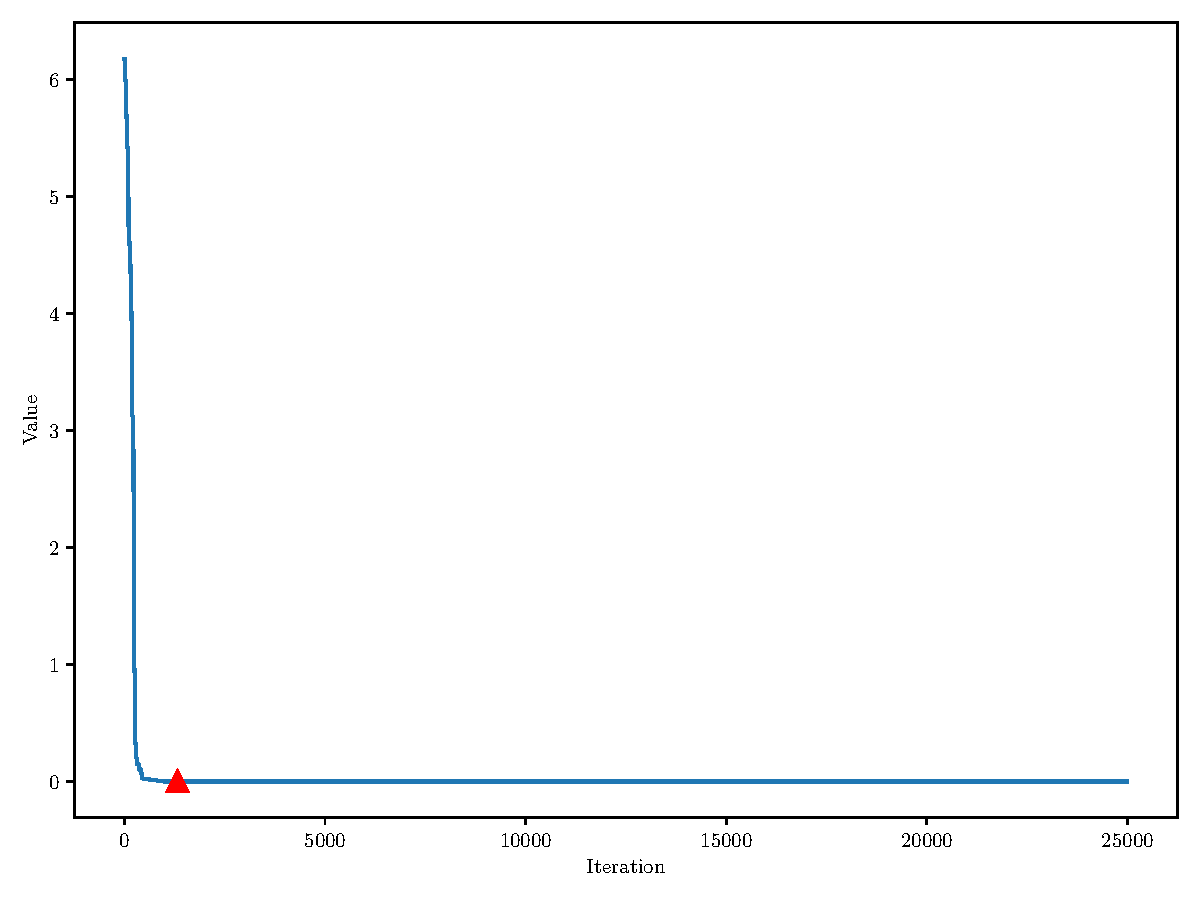
\includegraphics[width=\textwidth]{figures/Random Search_loss.pdf}
        \caption{最优值收敛曲线}
    \end{subfigure}
    \begin{subfigure}{0.4\textwidth}
        \centering
        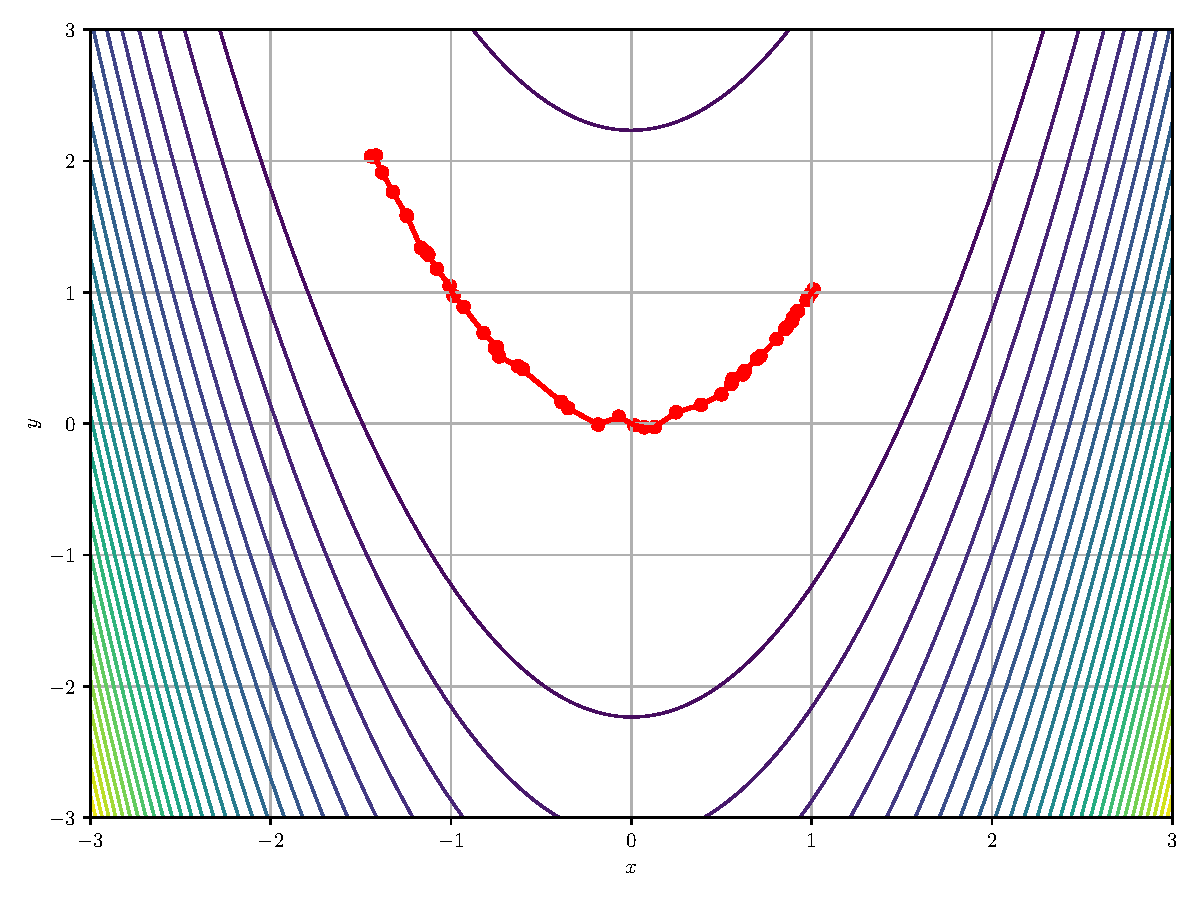
\includegraphics[width=\textwidth]{figures/Random Search_points.pdf}
        \caption{最优点收敛路径}
    \end{subfigure}
    \caption{Random Search的最优值收敛曲线与最优点收敛路径}
    \label{figure:random search}
\end{figure}
\begin{figure}[!ht]
    \centering
    \begin{subfigure}{0.4\textwidth}
        \centering
        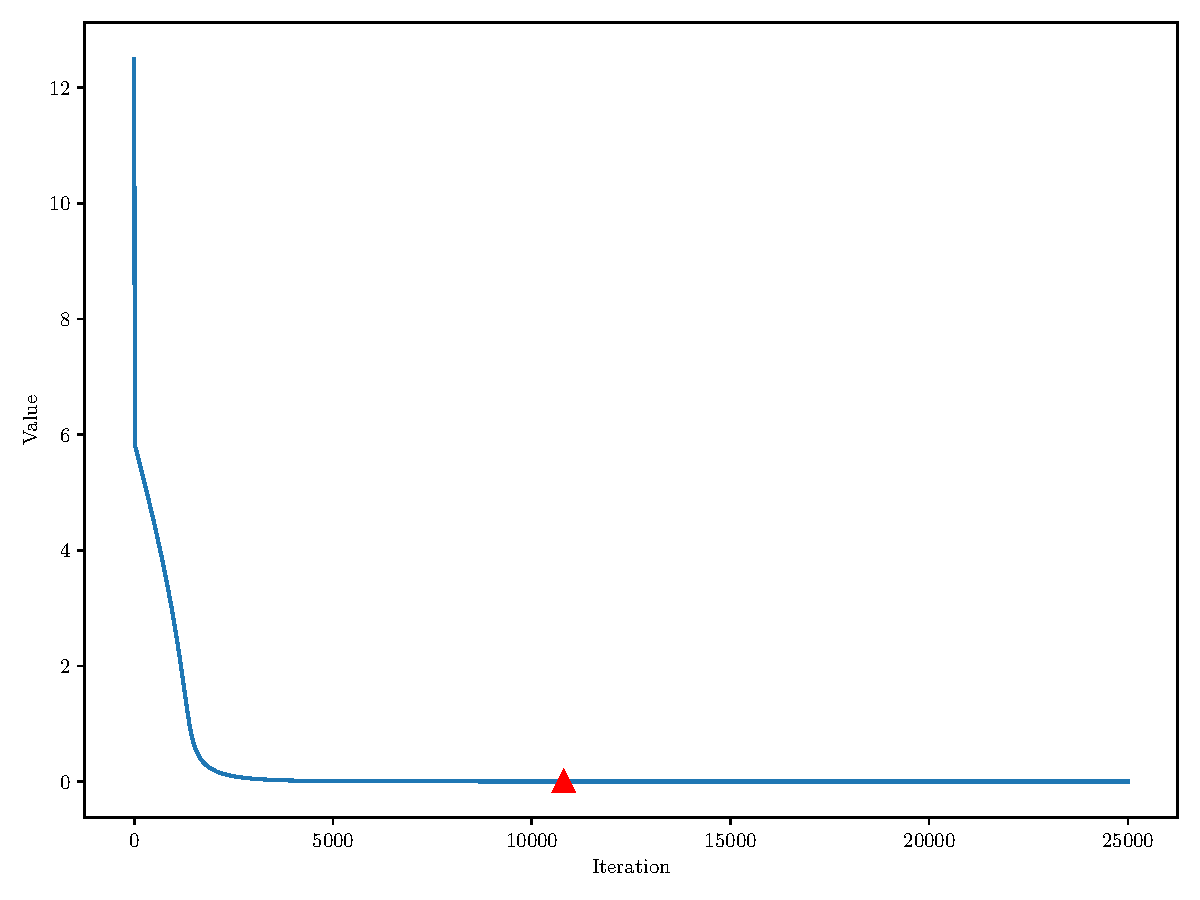
\includegraphics[width=\textwidth]{figures/Gradient Descent_loss.pdf}
        \caption{最优值收敛曲线}
    \end{subfigure}
    \begin{subfigure}{0.4\textwidth}
        \centering
        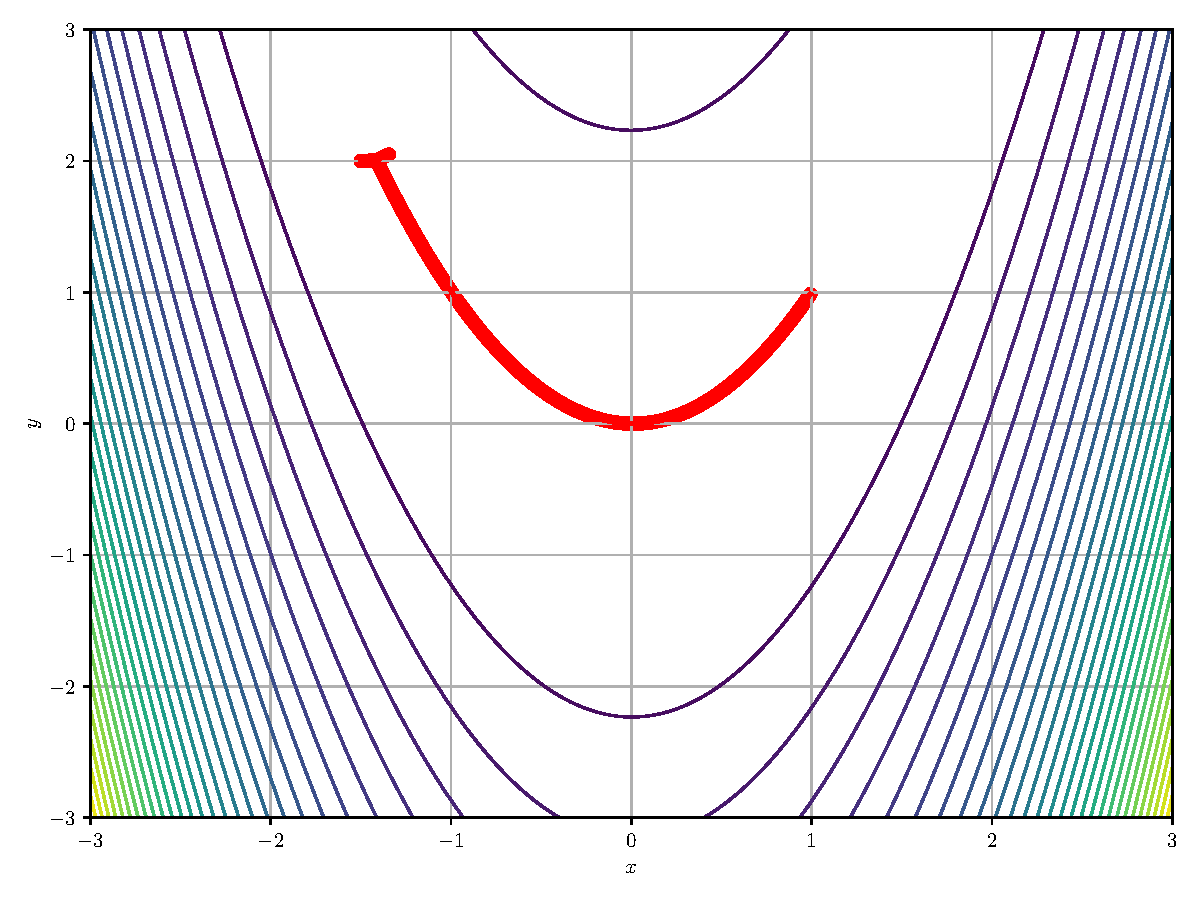
\includegraphics[width=\textwidth]{figures/Gradient Descent_points.pdf}
        \caption{最优点收敛路径}
    \end{subfigure}
    \caption{Gradient Descent的最优值收敛曲线与最优点收敛路径}
\end{figure}
\begin{figure}[!ht]
    \centering
    \begin{subfigure}{0.4\textwidth}
        \centering
        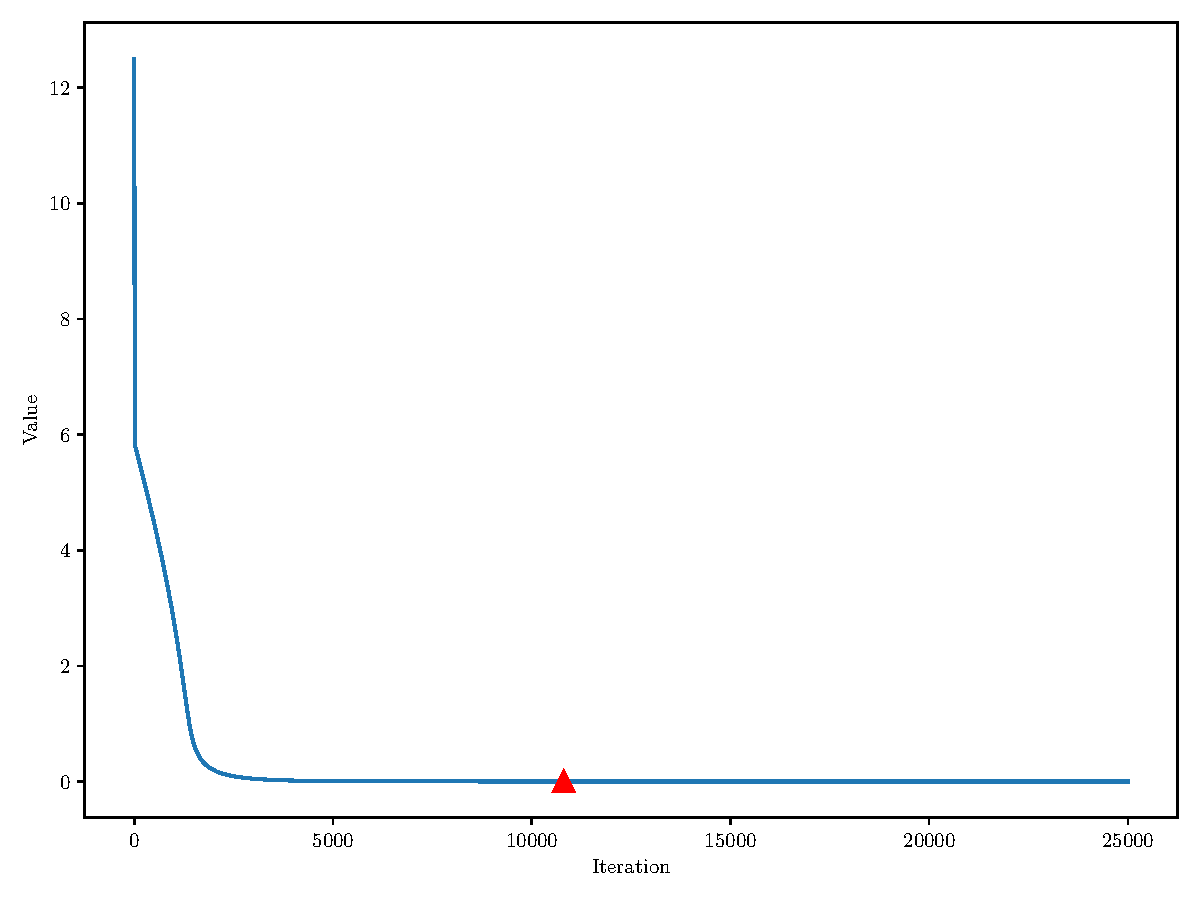
\includegraphics[width=\textwidth]{figures/Subgradient Descent_loss.pdf}
        \caption{最优值收敛曲线}
    \end{subfigure}
    \begin{subfigure}{0.4\textwidth}
        \centering
        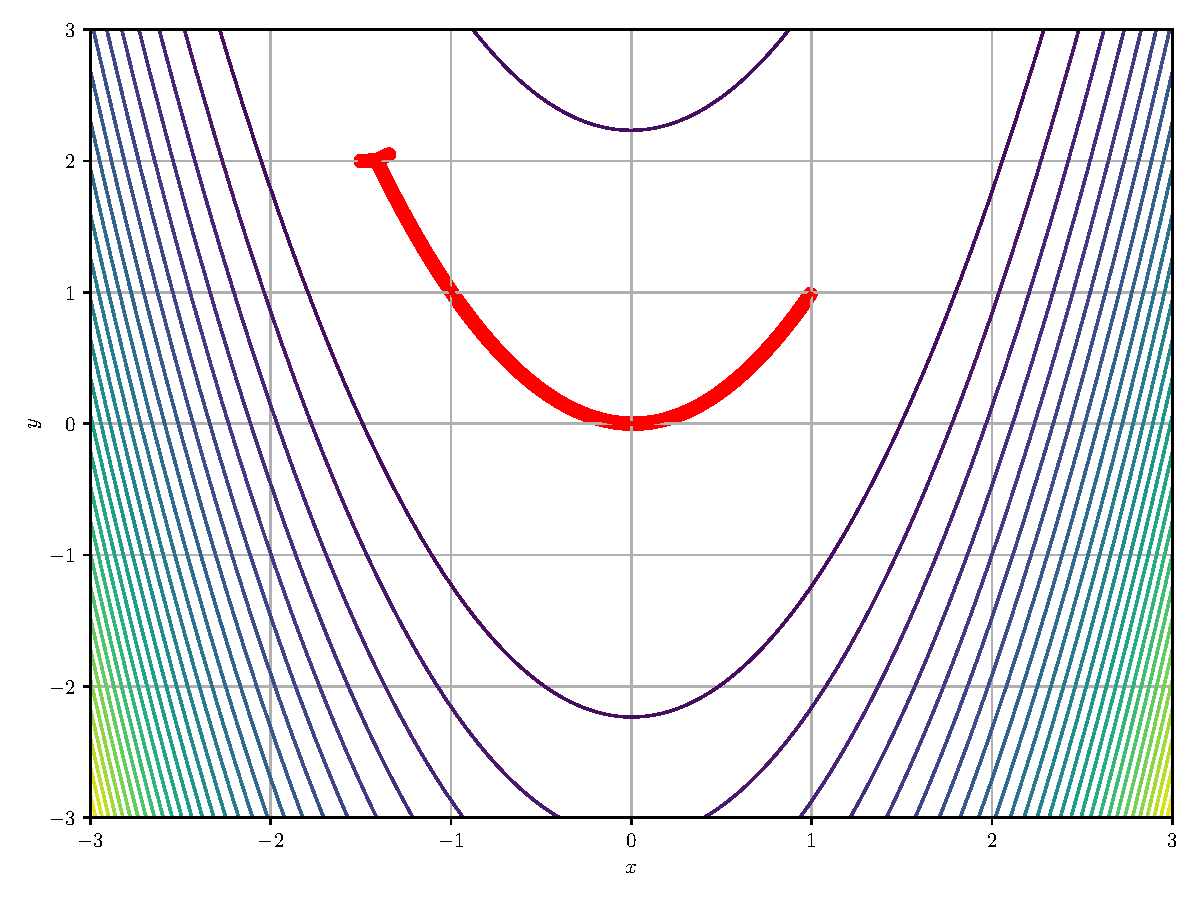
\includegraphics[width=\textwidth]{figures/Subgradient Descent_points.pdf}
        \caption{最优点收敛路径}
    \end{subfigure}
    \caption{Subgradient Descent的最优值收敛曲线与最优点收敛路径}
\end{figure}
\begin{figure}[!ht]
    \centering
    \begin{subfigure}{0.4\textwidth}
        \centering
        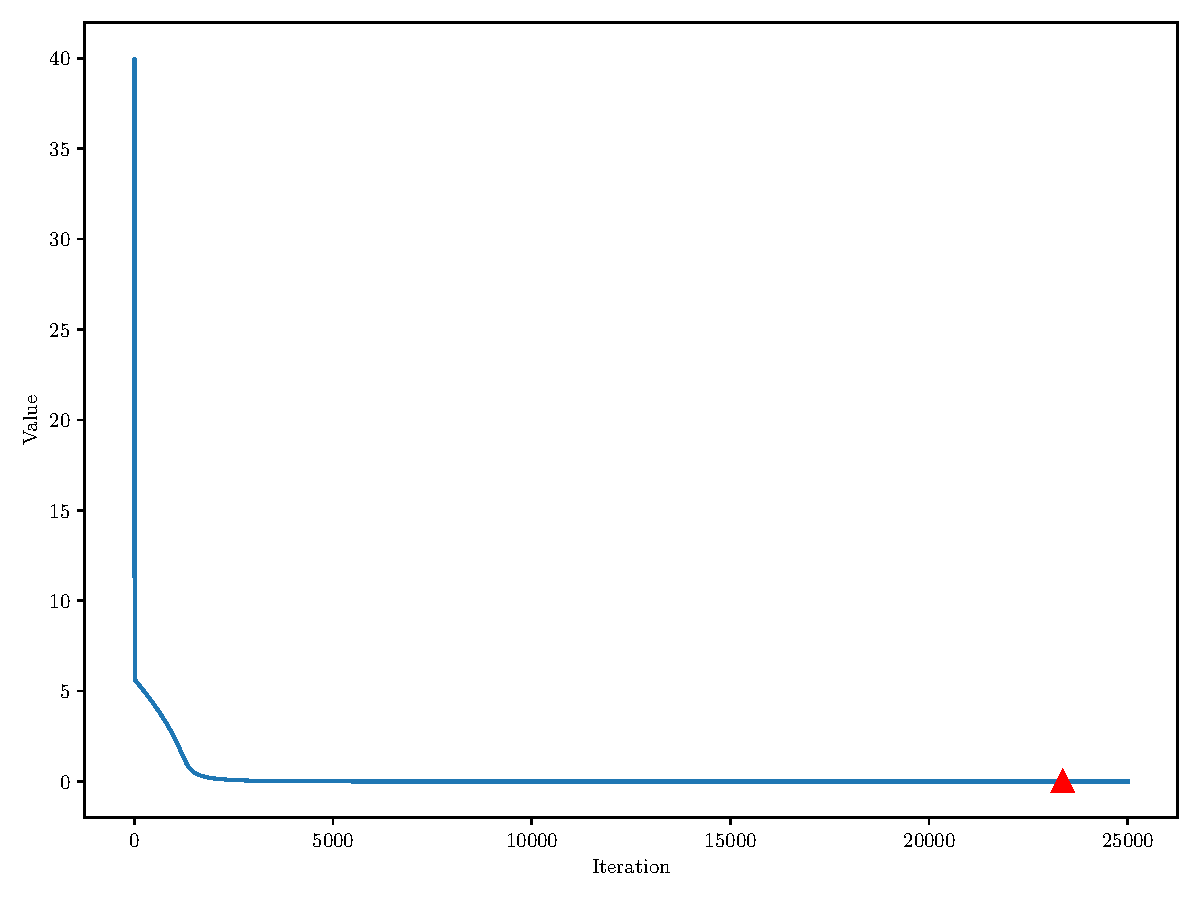
\includegraphics[width=\textwidth]{figures/Conjugate Direction_loss.pdf}
        \caption{最优值收敛曲线}
    \end{subfigure}
    \begin{subfigure}{0.4\textwidth}
        \centering
        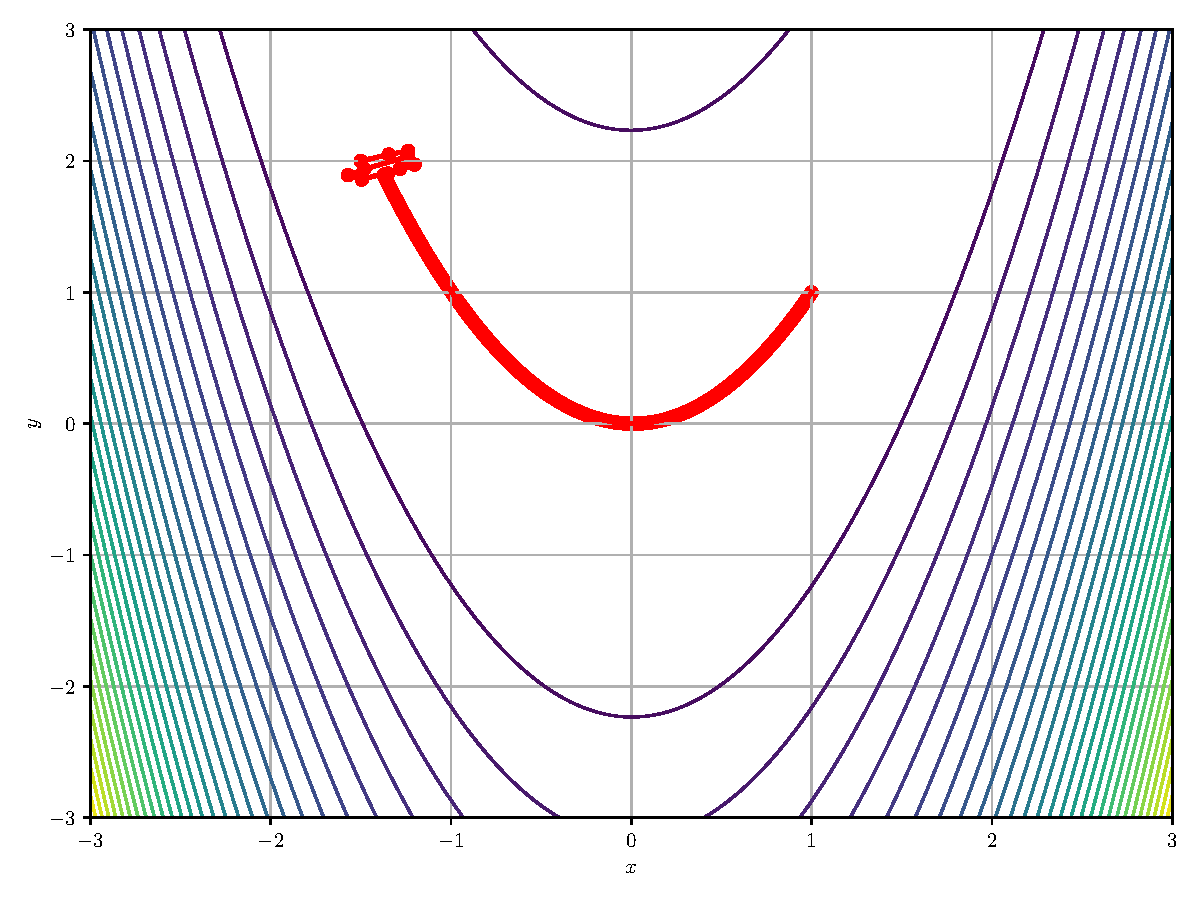
\includegraphics[width=\textwidth]{figures/Conjugate Direction_points.pdf}
        \caption{最优点收敛路径}
    \end{subfigure}
    \caption{Conjugate Direction的最优值收敛曲线与最优点收敛路径}
\end{figure}
\begin{figure}[!ht]
    \centering
    \begin{subfigure}{0.4\textwidth}
        \centering
        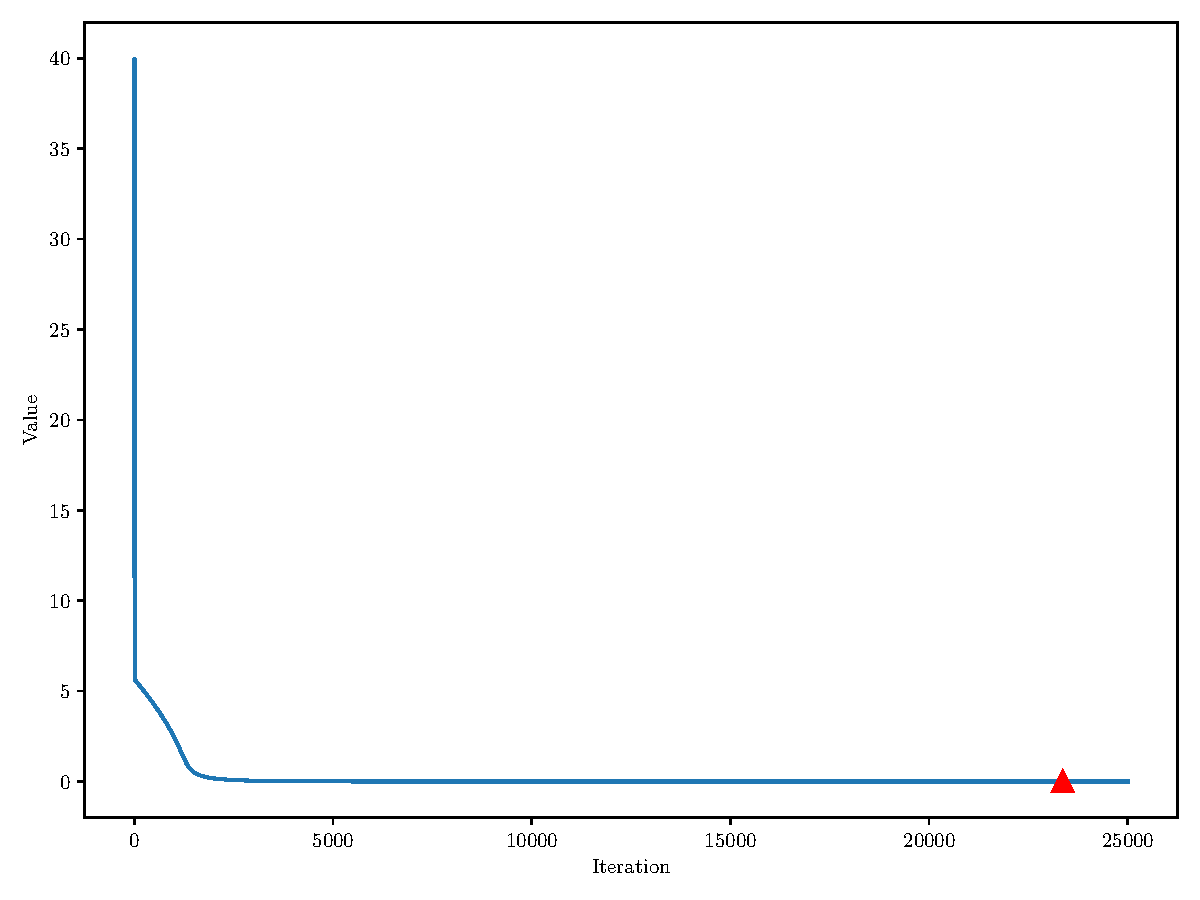
\includegraphics[width=\textwidth]{figures/Conjugate Gradient_loss.pdf}
        \caption{最优值收敛曲线}
    \end{subfigure}
    \begin{subfigure}{0.4\textwidth}
        \centering
        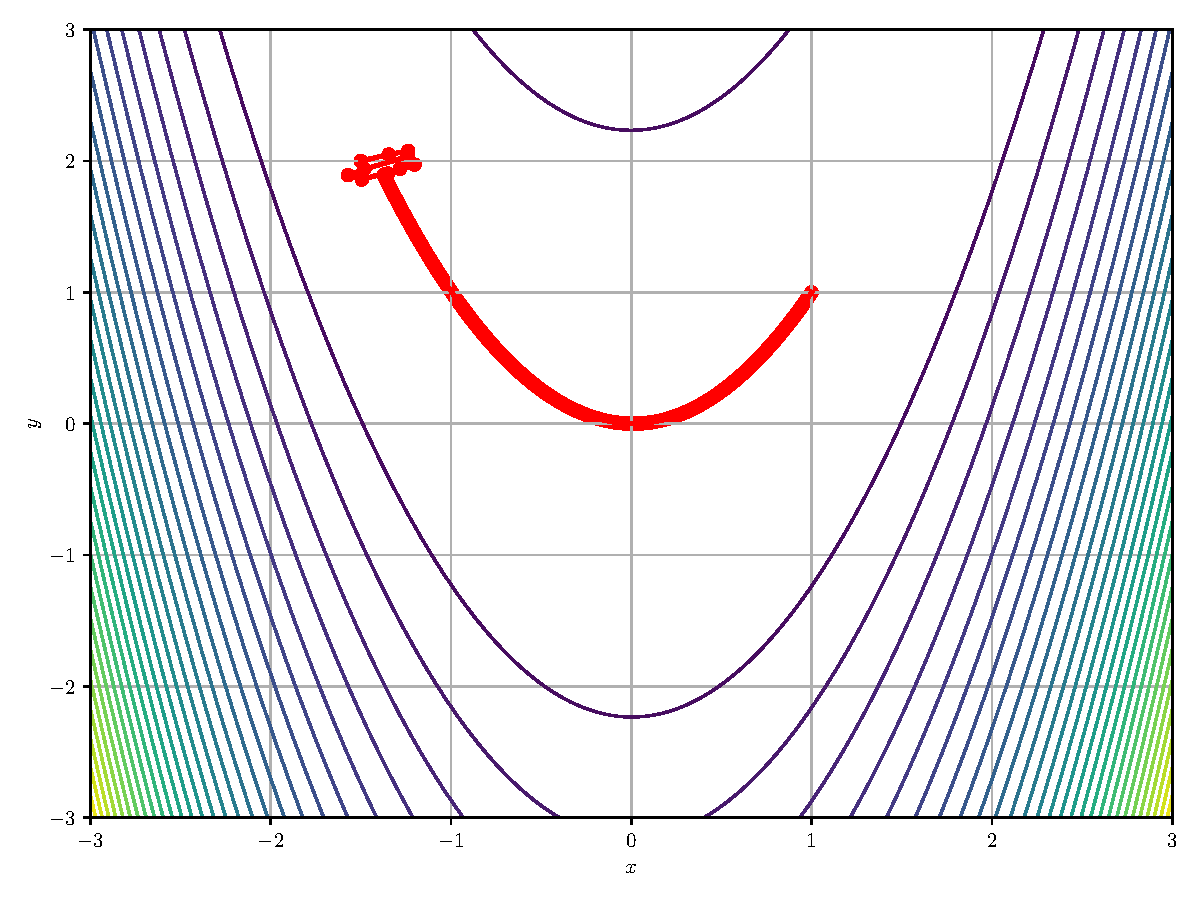
\includegraphics[width=\textwidth]{figures/Conjugate Gradient_points.pdf}
        \caption{最优点收敛路径}
    \end{subfigure}
    \caption{Conjugate Gradient的最优值收敛曲线与最优点收敛路径}
\end{figure}
\begin{figure}[!ht]
    \centering
    \begin{subfigure}{0.4\textwidth}
        \centering
        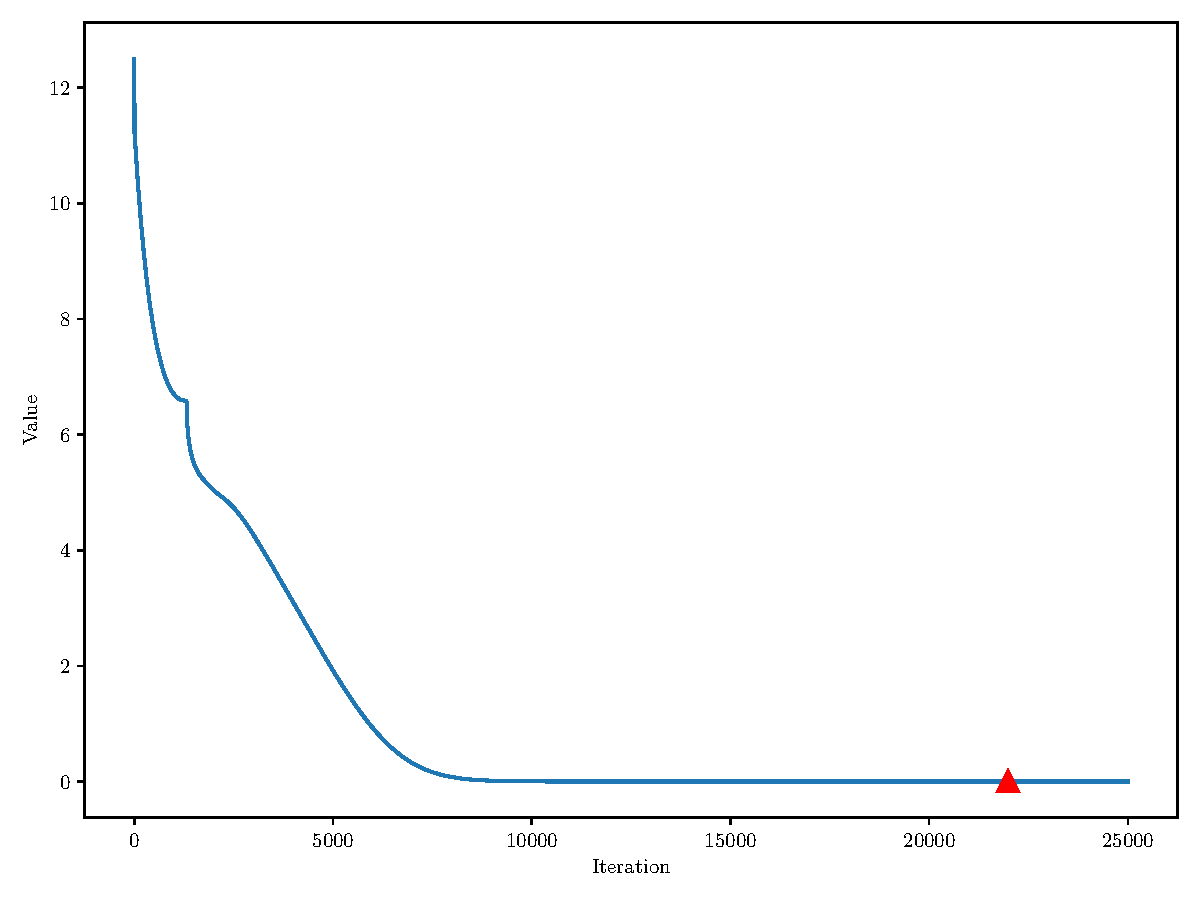
\includegraphics[width=\textwidth]{figures/BFGS_loss.pdf}
        \caption{最优值收敛曲线}
    \end{subfigure}
    \begin{subfigure}{0.4\textwidth}
        \centering
        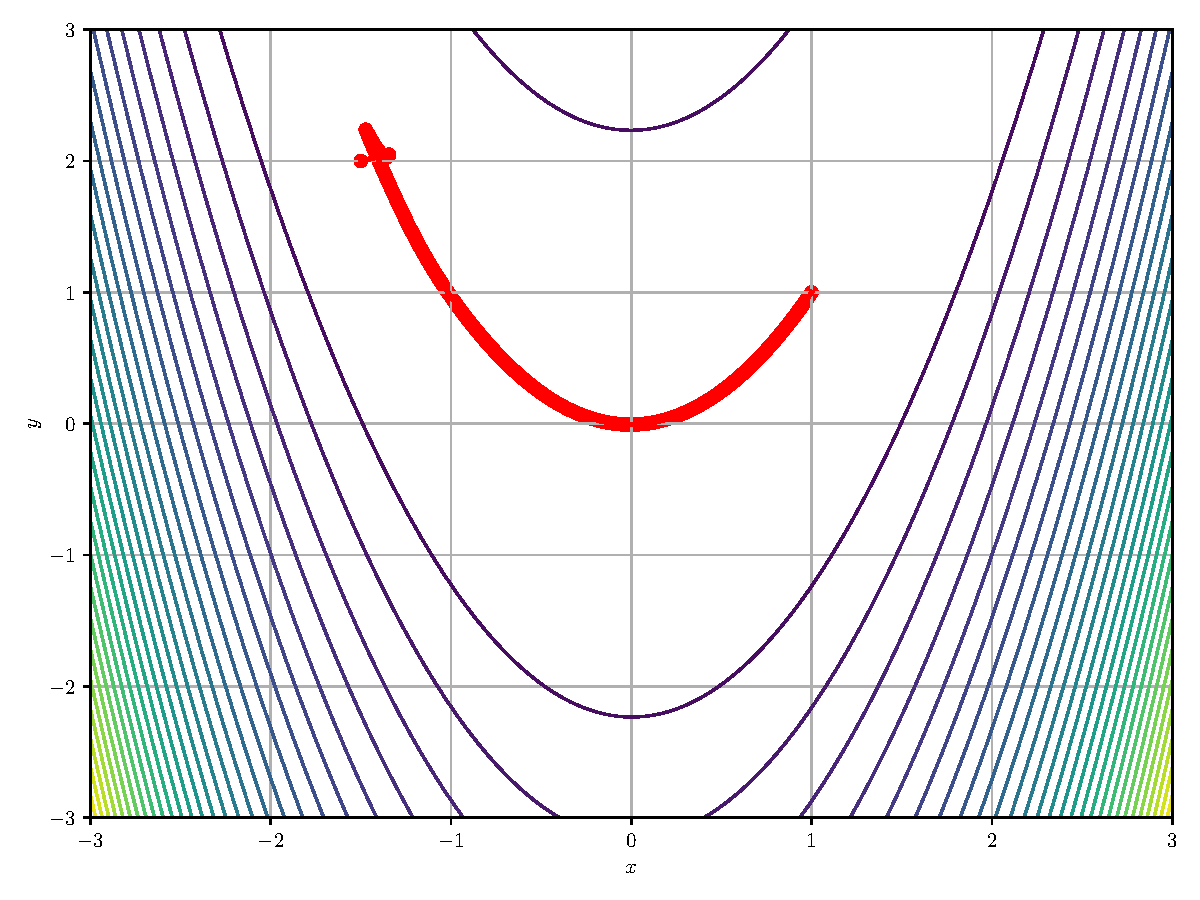
\includegraphics[width=\textwidth]{figures/BFGS_points.pdf}
        \caption{最优点收敛路径}
    \end{subfigure}
    \caption{BFGS的最优值收敛曲线与最优点收敛路径}
\end{figure}
\begin{figure}[!ht]
    \centering
    \begin{subfigure}{0.4\textwidth}
        \centering
        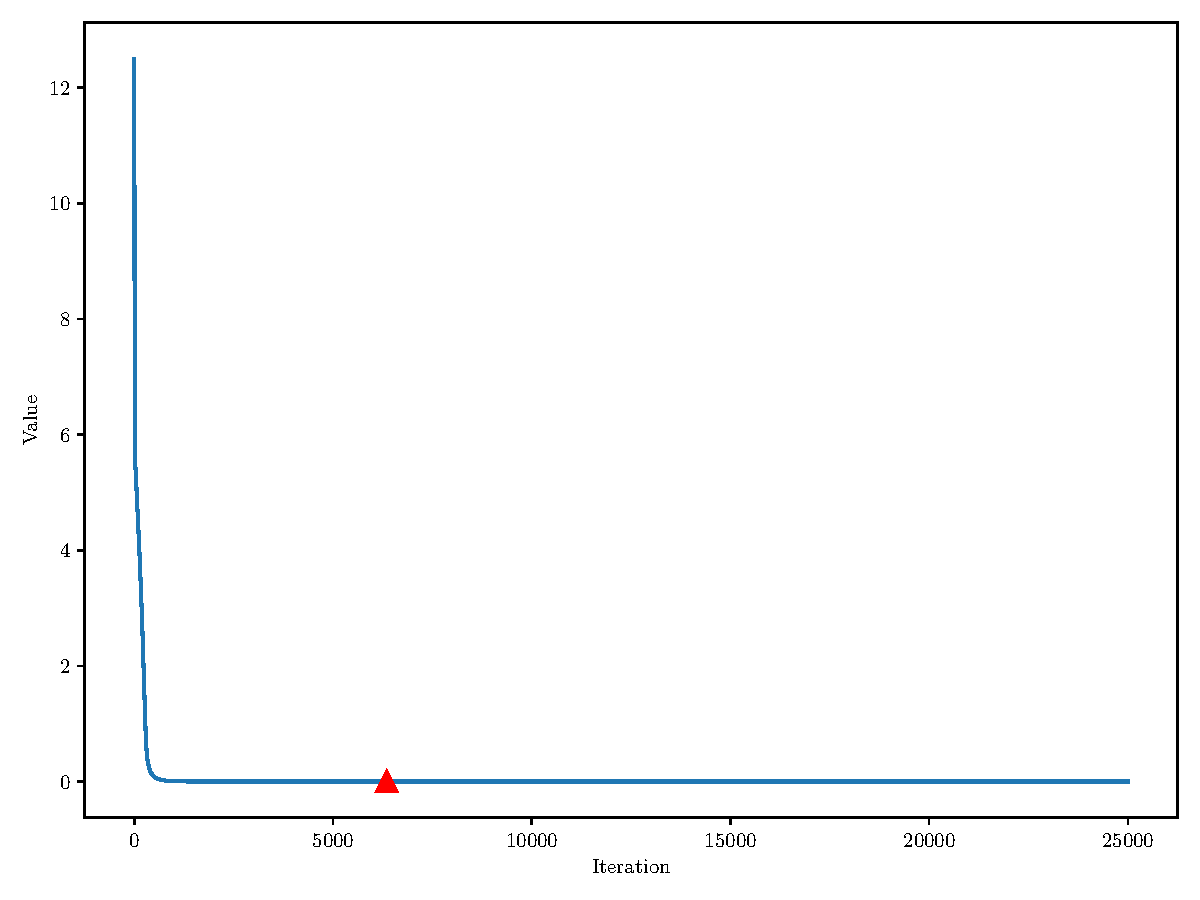
\includegraphics[width=\textwidth]{figures/SGD_loss.pdf}
        \caption{最优值收敛曲线}
    \end{subfigure}
    \begin{subfigure}{0.4\textwidth}
        \centering
        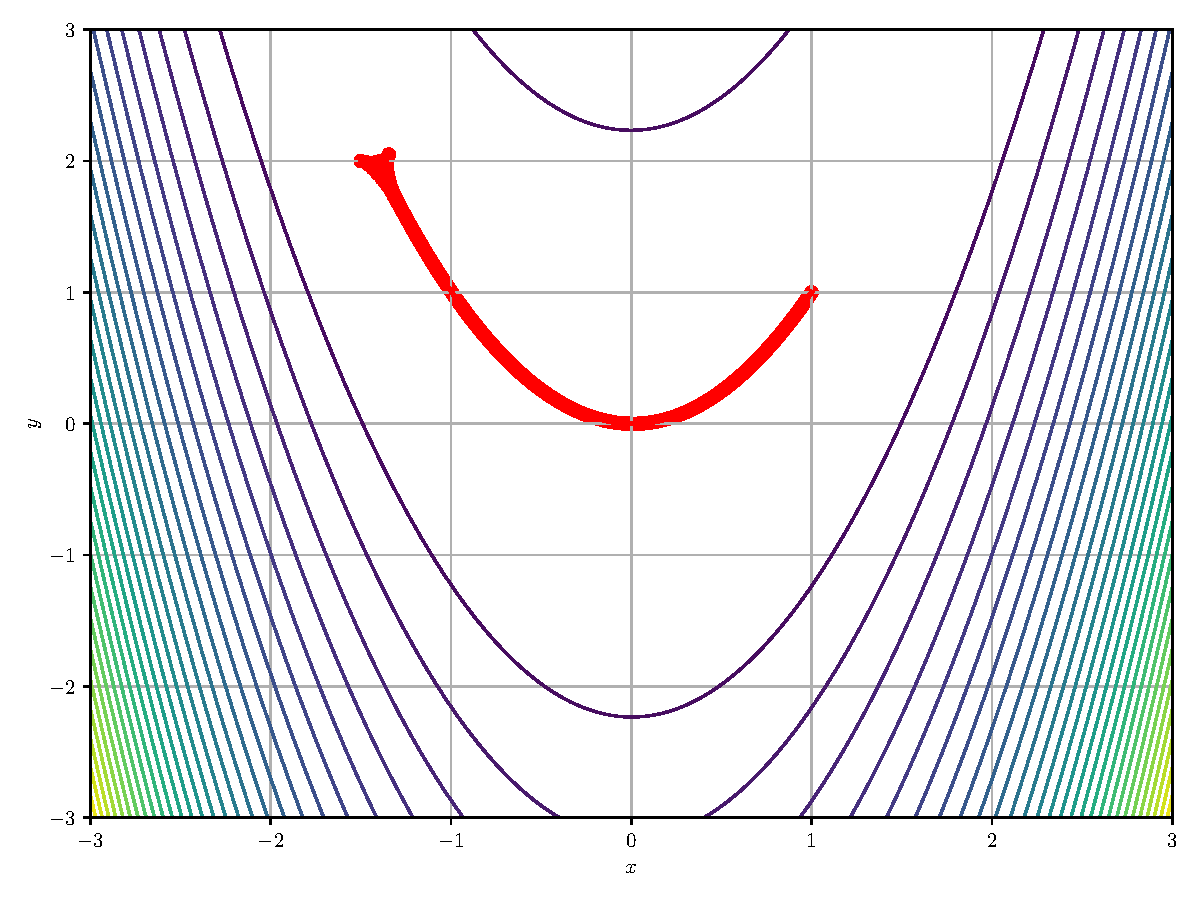
\includegraphics[width=\textwidth]{figures/SGD_points.pdf}
        \caption{最优点收敛路径}
    \end{subfigure}
    \caption{SGD的最优值收敛曲线与最优点收敛路径}
\end{figure}
\begin{figure}[!ht]
    \centering
    \begin{subfigure}{0.4\textwidth}
        \centering
        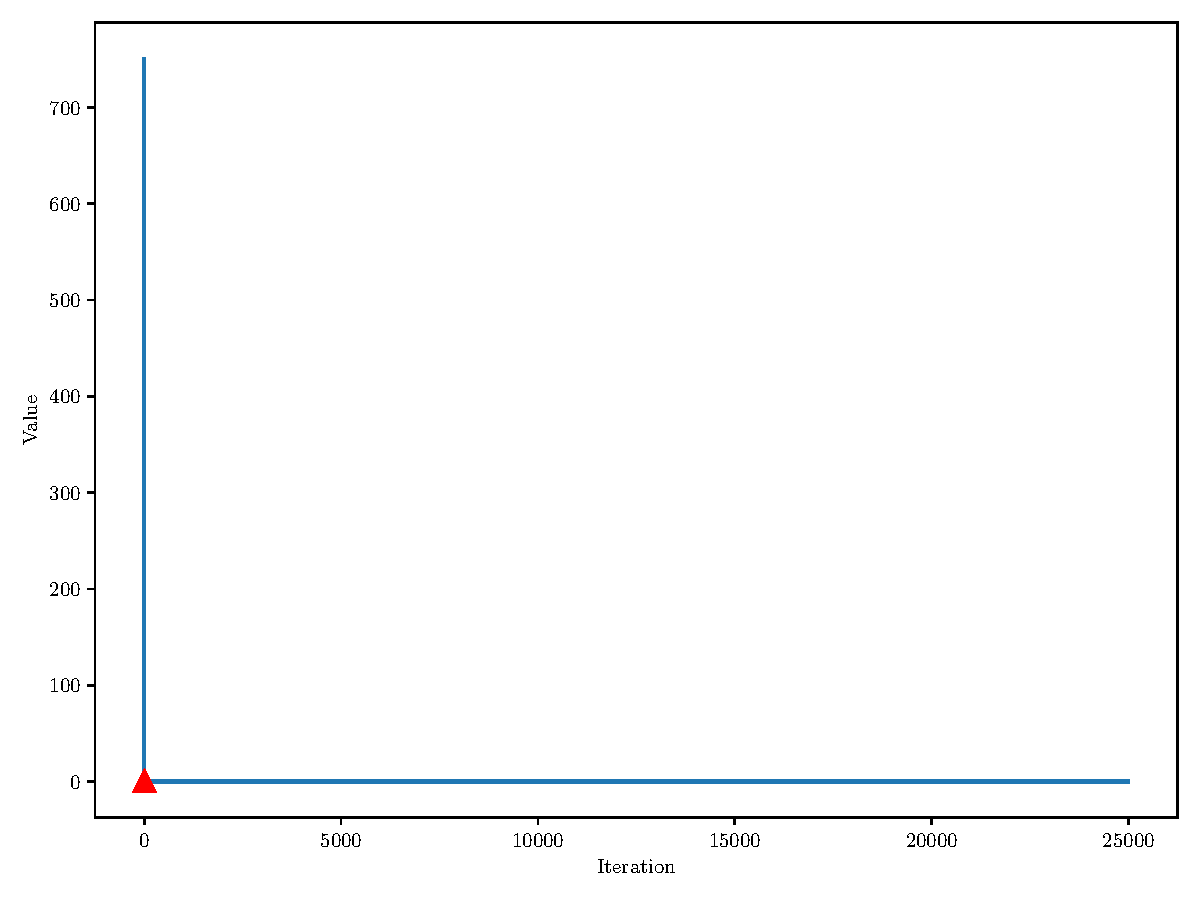
\includegraphics[width=\textwidth]{figures/Newton_loss.pdf}
        \caption{最优值收敛曲线}
    \end{subfigure}
    \begin{subfigure}{0.4\textwidth}
        \centering
        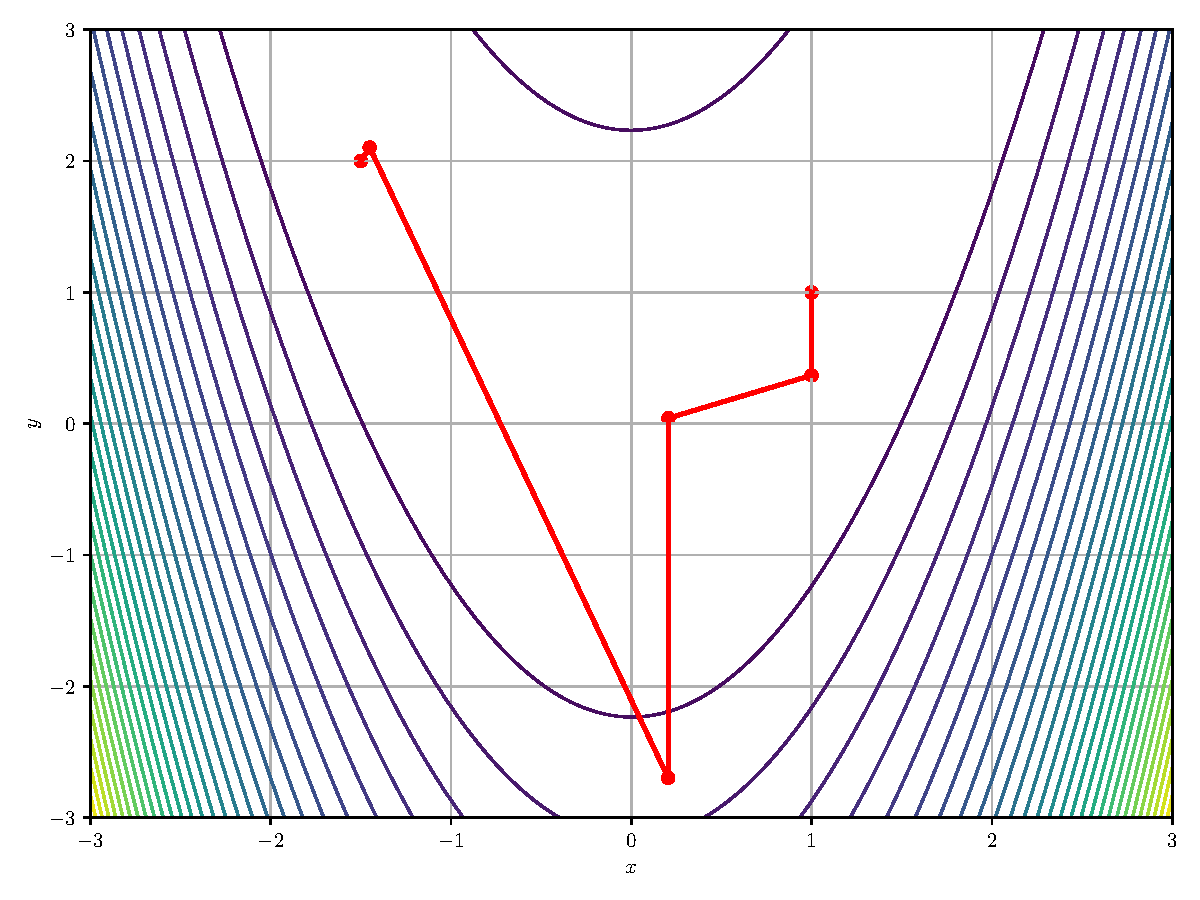
\includegraphics[width=\textwidth]{figures/Newton_points.pdf}
        \caption{最优点收敛路径}
    \end{subfigure}
    \caption{Newton的最优值收敛曲线与最优点收敛路径}
\end{figure}
\begin{figure}[!ht]
    \centering
    \begin{subfigure}{0.4\textwidth}
        \centering
        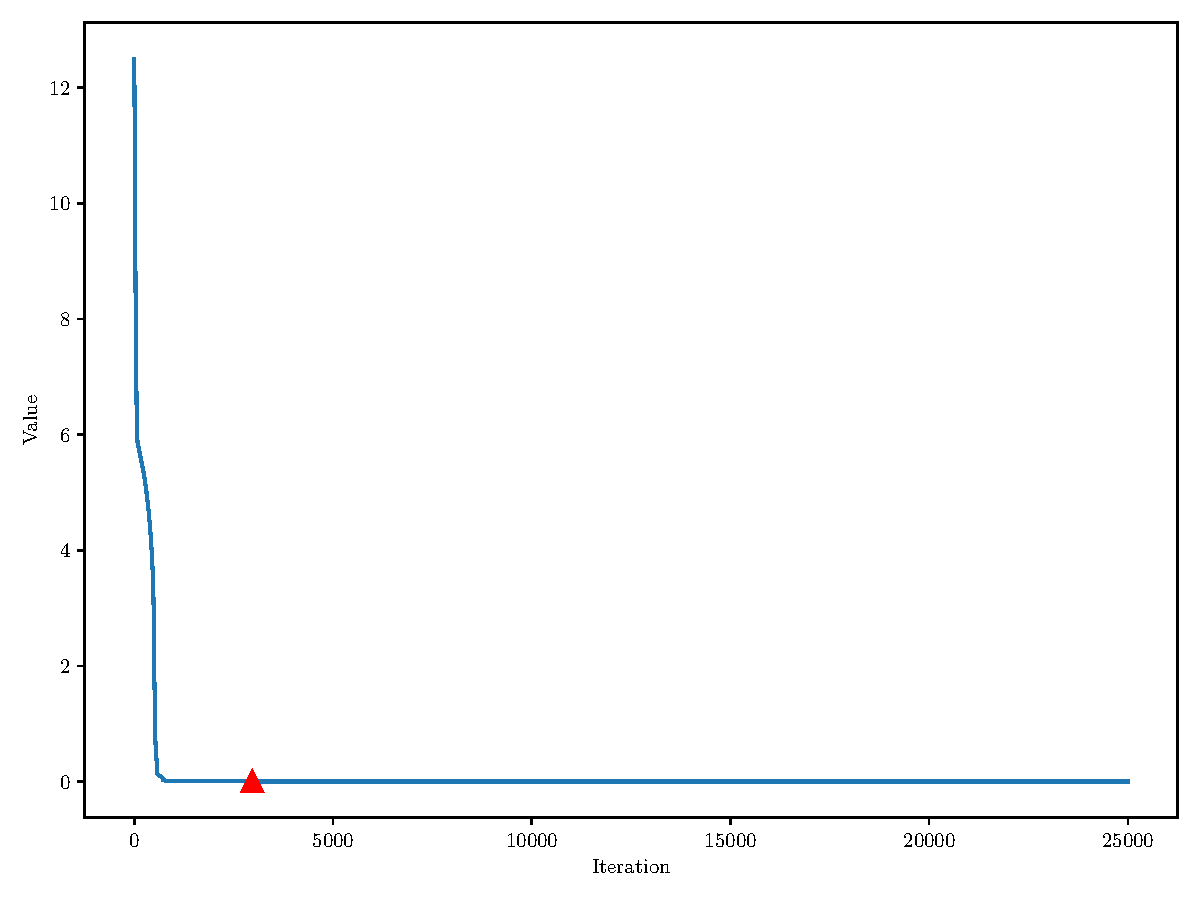
\includegraphics[width=\textwidth]{figures/Damped Newton_loss.pdf}
        \caption{最优值收敛曲线}
    \end{subfigure}
    \begin{subfigure}{0.4\textwidth}
        \centering
        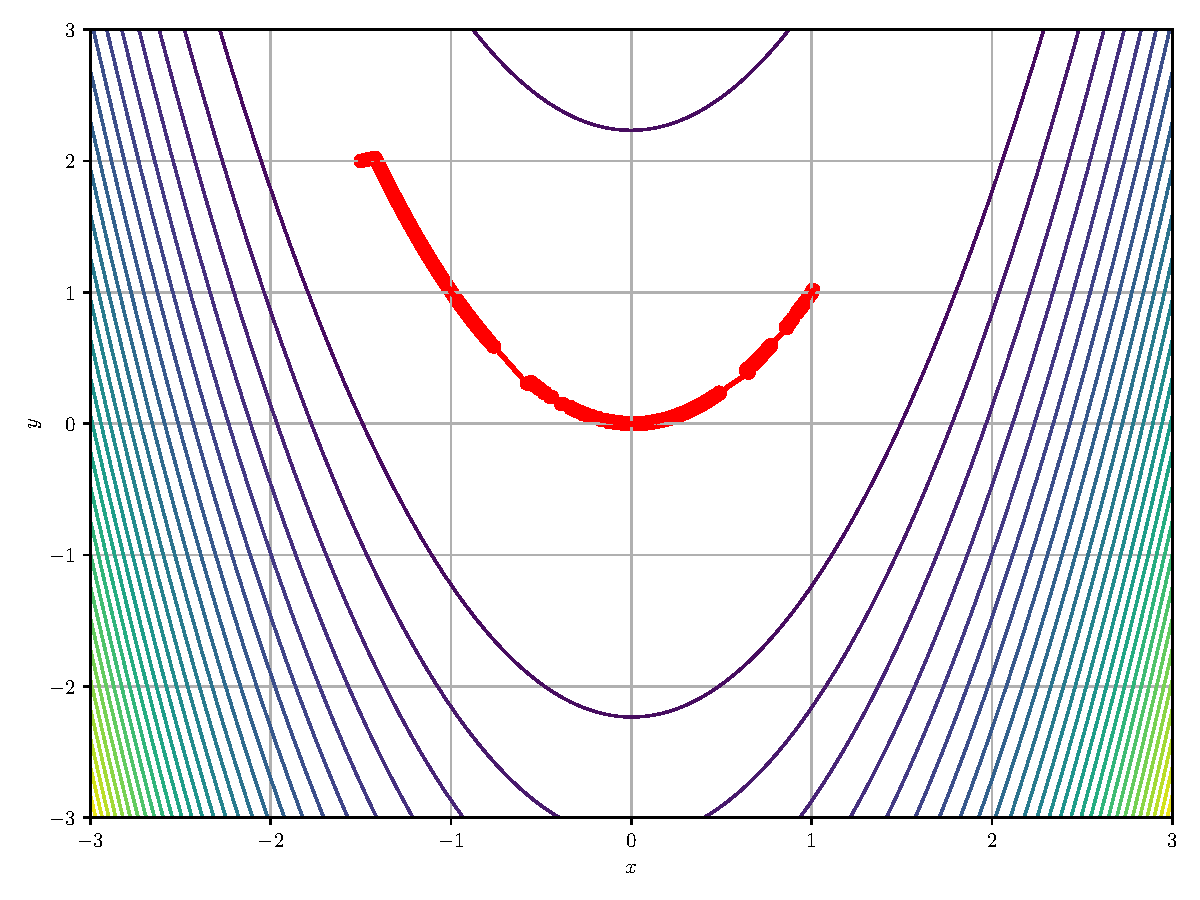
\includegraphics[width=\textwidth]{figures/Damped Newton_points.pdf}
        \caption{最优点收敛路径}
    \end{subfigure}
    \caption{Damped Newton的最优值收敛曲线与最优点收敛路径}
\end{figure}
\begin{figure}[!ht]
    \centering
    \begin{subfigure}{0.4\textwidth}
        \centering
        \includegraphics[width=\textwidth]{figures/ADMM_loss.pdf}
        \caption{最优值收敛曲线}
    \end{subfigure}
    \begin{subfigure}{0.4\textwidth}
        \centering
        \includegraphics[width=\textwidth]{figures/ADMM_points.pdf}
        \caption{最优点收敛路径}
    \end{subfigure}
    \caption{ADMM的最优值收敛曲线与最优点收敛路径}
\end{figure}
\begin{figure}[!ht]
    \centering
    \begin{subfigure}{0.4\textwidth}
        \centering
        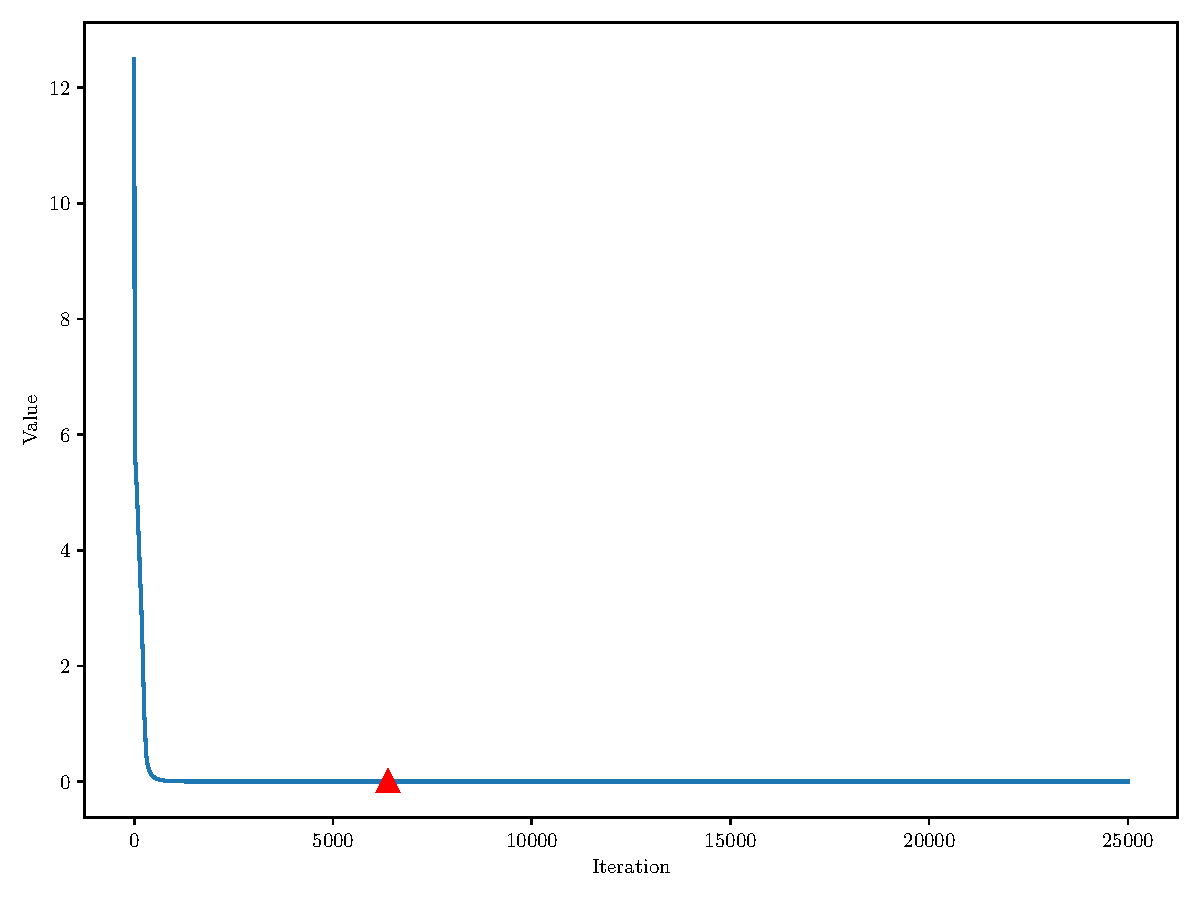
\includegraphics[width=\textwidth]{figures/Krylov_loss.pdf}
        \caption{最优值收敛曲线}
    \end{subfigure}
    \begin{subfigure}{0.4\textwidth}
        \centering
        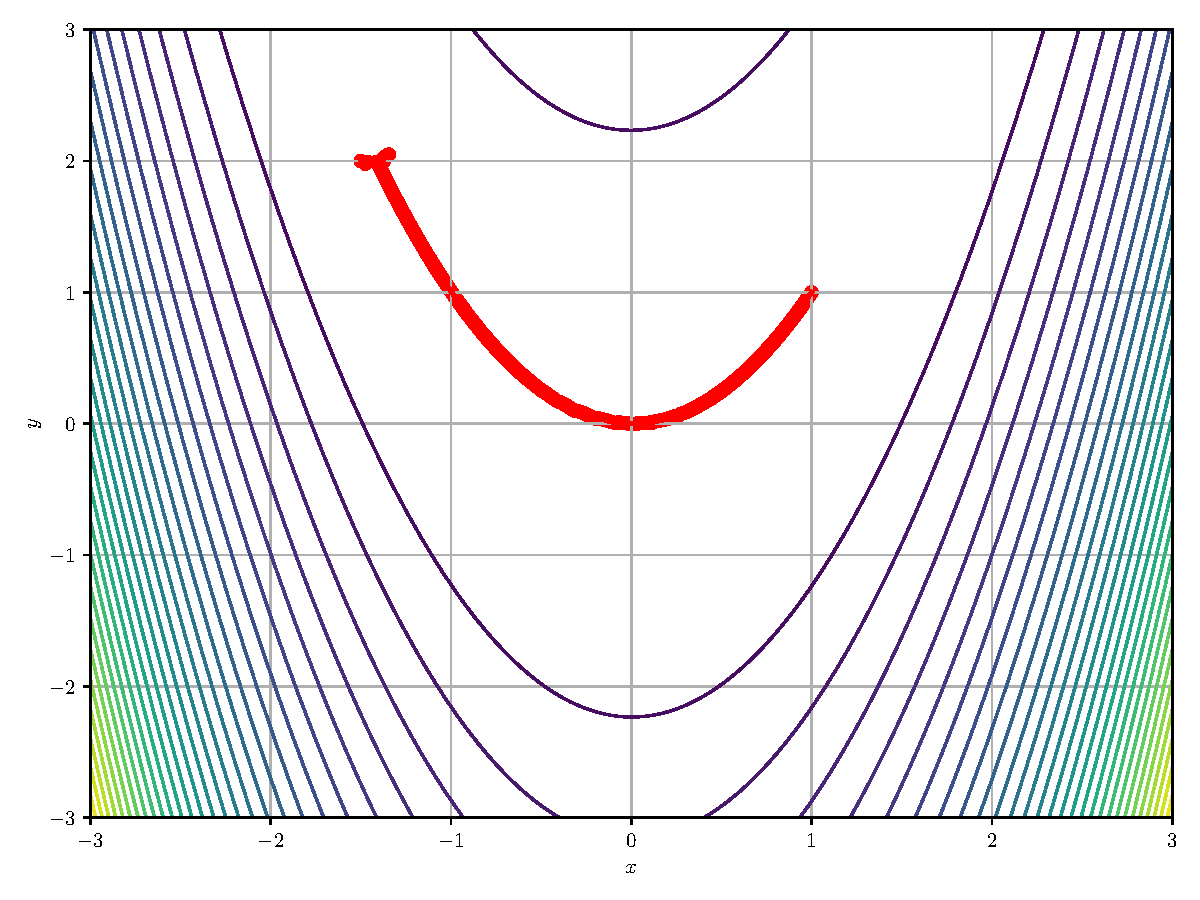
\includegraphics[width=\textwidth]{figures/Krylov_points.pdf}
        \caption{最优点收敛路径}
    \end{subfigure}
    \caption{Krylov的最优值收敛曲线与最优点收敛路径}
    \label{figure:krylov}
\end{figure}

从各图可看出,各优化器均在较少的迭代轮次内下降至最优值附近,但各优化器迭代至最优点需要的迭代轮次总和不同。
综合\cref{table:result}可知,Newton法所需要的迭代轮次最少。

鉴于Random Search优化器对初始随机种子较为敏感,实验对多个随机种子进行了实验比较,结果显示使用种子42时所需迭代轮次较少,因此在实验中固定采用该种子。

从\cref{figure:random search}中可看出,Random Search优化器也在较少的迭代轮次下收敛到最优点。

    % \section{核心优化思想及其发展历程}

\subsection{优化思想}

为了在多个域(如物理域、网络域等)上同时优化预测性能,文章使用了多任务学习(Multi-Task Learning, MTL)\cite{ruder2017overviewmultitasklearningdeep}方法,其目标是联合优化每个任务的损失
\begin{equation*}
    \min_{\bm{W}_s,\bm{W}_1,\bm{W}_2,\cdots,\bm{W}_D}\sum_{d=1}^D\beta_d\mathcal{L}_d(\bm{W}_s,\bm{W}_d) \text{,}
\end{equation*}
其中$\bm{W}_s$为共享层参数,$\bm{W}_d$、$\mathcal{L}_d$和$\beta_d$分别为第$d$域的专属参数、损失函数及任务权重。

为了解决梯度冲突问题,引入了多梯度下降算法(Multiple Gradient Descent Algorithm,MGDA)\cite{desideri2012multiple},其基本思想是寻找一组权重$\{\gamma_d\}$,使得多个损失函数在共享参数$\bm{W}_s$上的梯度方向可以共同优化,即
\optmodule{\min_{\gamma_1,\gamma_2,\cdots,\gamma_D}}{\left\|\sum_{d=1}^D\gamma_d\nabla_{\bm{W}_s}\mathcal{L}_d(\bm{W}_s,\bm{W}_d)\right\|^2}{
    &\sum_{d=1}^D\gamma_d=1\text{,} \\
    &\gamma_1,\gamma_2,\cdots,\gamma_D\geq0\text{,}
    \label{equation:MGDA}
}
该优化问题保证在共享参数更新中不会偏向某一特定任务。

当$D=2$时,\cref{equation:MGDA}简化为
\optmodule*{\min_{\gamma}}{\left\|\gamma\nabla_{\bm{W}_s}\mathcal{L}_1(\bm{W}_s,\bm{W}_1)+(1-\gamma)\nabla_{\bm{W}_s}\mathcal{L}_2(\bm{W}_s,\bm{W}_2)\right\|^2}{
    &\gamma\geq0\text{。}
}

\subsection{MTL的发展历程}

多任务学习的思想可以追溯到上世纪90年代,其中最具代表性的开创性工作来自于Rich Caruana在1997年的论文\cite{caruana1997multitask}。
这篇文章明确提出了一个基本设想:如果我们同时学习多个相互关联的任务,就可以通过共享表示来提升模型的泛化能力。
这一时期的多任务学习主要关注于参数共享的形式,也就是通过设计模型结构,让多个任务共享一部分网络参数(例如前几层),而在高层则保留各自的特定参数。
这样的设计既利用了任务间的相关性,又保留了个性化特征。

随着深度学习的发展,特别是CNN和RNN等结构的广泛应用,多任务学习进入了“深度MTL”时代。
研究者开始思考不仅仅是共享前几层的问题,而是如何更加灵活地在网络中进行共享。
例如,Cross-Stitch Networks\cite{misra2016cross}、Sluice Networks\cite{ruder2019latent}等进一步提出了“选择性共享”的策略,即网络的每一层都可以决定是否共享,这种方式使得模型在面对任务相关性强弱不一的场景时具有更大的灵活性。

但是,这一时期很快暴露出一个重要问题:共享结构设计虽然能够在一定程度上提高性能,但很多时候,多任务学习的训练过程并不稳定。
有时候,模型在优化某个任务时,会影响甚至破坏另一个任务的性能。这种现象在训练过程中表现为任务之间的“负迁移”或“梯度冲突”。
任务的损失函数虽然在理论上可以共同最小化,但在梯度空间中,它们的方向可能是彼此冲突的。
这就催生了人们对多任务优化策略本身的深入研究。

真正把这个问题提升到理论高度的是文章\cite{desideri2012multiple,sener2018multi}。
文章将多任务学习转化为一个经典的多目标优化问题(Multi-objective Optimization, MOO),即在参数空间中同时最小化多个目标函数,而不是对它们进行简单的加权求和。
他们引入了Pareto最优的概念,认为多任务学习的本质是找到一个所有任务都“无法进一步改善而不损害其他任务”的平衡点。

MGDA 的核心思想是,每次参数更新时都不直接沿着所有梯度简单平均的方向走,而是求解一个最小范数问题,在所有任务的梯度凸包中找到一个合适的组合方向,使得整体更新方向在几何意义上最“中性”、最“折中”。
这个方向被视为当前任务之间最合理的优化方向,从而避免了梯度冲突的直接影响。
该方法提出后,迅速成为多任务优化的核心代表方法之一。

到今天,多任务学习已经不再只是“如何共享参数”这样一个模型结构设计问题,更是一个“如何优化更新”的动态策略问题。
MGDA作为第一个明确从优化角度重新定义MTL训练流程的方法,为后续梯度调度类方法打开了方向,构建了以“Pareto最优”为核心思想的全新视角。

    % \section{实验设置、数据集及结果分析}

文章使用SWaT(Secure Water Treatment)\cite{mathur2016swat}数据集进行实验。
该数据集由新加坡科技设计大学(Singapore University of Technology and Design,SUTD)网络安全研究中心的iTrust实验室发布,模拟了真实水处理系统的运行场景。
数据集包含51个物理传感器(如流量计、阀门状态)和16个网络特征(如数据包数量、协议类型),时间跨度为11天,前7天为正常操作,后4天注入41种攻击。
\cref{table:swat static info}总结了SWaT数据集在物理和网络领域的统计数据。

文章使用准确率(Precision)、召回率(Recall)、假阳性率(False Positive Rate,FPR)和F1分数评估模型性能,这些指标的计算公式如下:
\begin{align*}
    &\mathrm{Precision}=\frac{\mathrm{TP}}{\mathrm{TP}+\mathrm{FP}} \text{,} \\
    &\mathrm{Recall}=\frac{\mathrm{TP}}{\mathrm{TP}+\mathrm{FN}} \text{,} \\
    &\mathrm{FPR}=\frac{\mathrm{FP}}{\mathrm{FP}+\mathrm{TN}} \text{,} \\
    &\mathrm{F1}=\frac{2\times\mathrm{Precision}\times\mathrm{Recall}}{\mathrm{Precision}+\mathrm{Recall}} \text{。}
\end{align*}
实验结果如\cref{table:matrics of mgdn and the baseline methods}所示。

\begin{table}[ht]
    \centering
    \caption{SWaT数据集在不同域中的统计数据}
    \label{table:swat static info}
    \begin{tabular}{ccccc}
        \toprule
        \textbf{域} & \textbf{训练数据} & \textbf{训练数据条目} & \textbf{特征数} & \textbf{异常率} \\
        \midrule
        物理域 & 21,830 & 34,201 & 51 & 16.61\% \\
        网络域 & 21,830 & 34,201 & 3  & 16.61\% \\
        \bottomrule
    \end{tabular}
\end{table}

\begin{table}[ht]
    \centering
    \caption{MGDN与基线方法的评价指标}
    \label{table:matrics of mgdn and the baseline methods}
    \begin{tabular}{ccccc}
        \toprule
        \textbf{Method} & \textbf{FPR (\%)} & \textbf{Precision (\%)} & \textbf{Recall (\%)} & \textbf{F1 (\%)} \\
        \midrule
        DTAAD       & 13.33 & 59.88 & 99.99 & 74.90 \\
        GDN         & 10.70 & 64.91 & 99.45 & 78.55 \\
        LSTM-AD     & 13.33 & 59.88 & 99.99 & 74.90 \\
        MAD-GAN     & 13.57 & 59.45 & 99.99 & 74.57 \\
        MSCRED      & 13.33 & 59.89 & 99.99 & 74.91 \\
        MTAD-GAT    & 13.39 & 59.78 & 99.99 & 74.83 \\
        OmniAnomaly & 13.36 & 59.83 & 99.99 & 74.87 \\
        TranAD      & 13.35 & 59.85 & 99.99 & 74.88 \\
        USAD        & 13.26 & 60.02 & 99.99 & 75.01 \\
        \textbf{MGDN}   & \textbf{3.07} & \textbf{84.65} & \textbf{85.12} & \textbf{84.88} \\
        \bottomrule
    \end{tabular}
\end{table}

\begin{table}[!ht]
    \centering
    \caption{不同多目标优化器下的评价指标}
    \label{table:matrics of opt}
    \begin{tabular}{cccc}
        \toprule
        \textbf{Method} & \textbf{Precision (\%)} & \textbf{Recall (\%)} & \textbf{F1 (\%)} \\
        \midrule
        0.25, 0.75  & 49.30 & 84.46 & 62.28 \\
        0.5, 0.5    & 83.15 & 82.34 & 83.87 \\
        0.75, 0.25  & 80.99 & 83.39 & 82.79 \\
        \textbf{MGDA}        & \textbf{84.65} & \textbf{85.12} & \textbf{84.88} \\
        \bottomrule
    \end{tabular}
\end{table}

将多梯度优化器更换成基于静态权重的梯度优化器,并分别设置不同的权重。
从\cref{table:matrics of opt}中可以看出,将物理域和网络域的损失权重分别设定为0.5和0.5能够取得比其他静态权重方法更好的效果,但仍然比使用MGDA的模型的F1低1.01\%。
因此,引入多梯度下降优化算法有利于模型更好地动态调整。

    % \section{结论}

文章提出了一种基于跨域表示学习的异常检测方法,该方法将多个域的ICS数据结合起来进行跨域学习和异常检测。
通过物理域与网络域数据的联合建模,克服了单领域分析的局限性。注意力机制与多任务优化的结合,使模型在保留领域特征的同时捕捉跨域关联。
文章在大规模的真实世界数据集上对模型进行了评估,实验结果表明文章的模型优于基准模型。
此外,文章的模型能够更好地平衡减少误报和提高异常检测精度之间的关系,提供了一个更实用和理想的ICS异常检测模型。


    % \stepcounter{section}
    % \renewcommand{\refname}{\chinese{section}、参考文献}

    % \phantomsection
    % \addcontentsline{toc}{section}{参考文献}
    % \bibliography{references}
\end{document}
